\documentclass{article}
\usepackage[utf8]{inputenc}
\documentclass[12pt,a4paper,portuges]{article}

\usepackage[utf8]{inputenc}
\usepackage[portuges]{babel}
\usepackage{graphicx}

\title{Relatório do Projeto de POO}
\author{António Chaves (A75870) \and Cesário Perneta (A73883) \and João Palmeira (A73864)}
\date{Maio 2016}

\begin{document}


\maketitle

\begin{figure}[!htb]
\centering

\includegraphics[scale=0.5] {imagens/Imagem3.jpg}
\end{figure}

\begin{figure}[!htb]
\centering

\includegraphics[scale=0.5] {imagens/Imagem2.jpg}
\end{figure}

\begin{figure}[!htb]
\centering

\includegraphics[scale=0.5] {imagens/Imagem1.jpg}
\end{figure}

\newpage

\tableofcontents

\newpage

\section{Introdução}

\paragraph{Neste trabalho foi proposto o desenvolvimento de uma aplicação que permita fazer a gestão de imóveis de uma imobliária contendo todos os dados sobre os imóveis, ou seja, desde a criação do imóvel no sistema até ao registo da venda do mesmo.}

\paragraph{Nesta aplicação podem-se registar dois tipos de utilizadores: os vendedores e os compradores.}

\paragraph{Os Vendedores podem inserir um anúncio, consultar todos os anúncios e remover qualquer um destes caso pretendam. Podem ainda alterar o estado de cada imóvel e têm acesso a vários tipos de informação tal como o número total de imóveis, total de visualizações de cada imóvel e o total de vendas.}

\paragraph{Os Compradores podem procurar determinado imóvel através de uma das suas característas ou encontrá-lo através de uma identificação (o id do imóvel). Têm permissão ainda para selecionar imóveis como favoritos, mas para isso necessitam de estar registados no sistema e desta forma têm acesso a um menu com opções gerais tal como o vendedor.}

\paragraph{Por último, este programa deverá permitir ao utilizador guardar num ficheiro de texto todo o tipo de informação que esteja em memória e o usuário deverá ter acesso ao que foi guardado novamente.}

\newpage

\section{Arquitetura de Classes Utilizadas}

\subsection{\textbf{Imoobiliaria}}

\paragraph{Esta é a classe mais importante da aplicação. Nela encontramos duas listas, nomeadamente, a lista de usuários (users) e a lista de todos os imóveis (imoveisGeral) bem como os principais menus: MenuInicial (menu inicial da aplicação, permite ao utilizador seleccionar a letra do comando que pretende inicializar. utilizando ainda funções que são apresentadas a seguir tais como MenuRegUtil e MenuInitSessao), MenuRegUtil (menu que permite registar um novo utilizador), MenuInitSessao (menu que permite que o utilizador inicie sessão na aplicação invocando a função iniciaSessao), MenuVendedor (menu criado para o vendedor que permite consultar informação própria do vendedor, pesquisar imóveis por preço e verificar as informações gerais), MenuComprador (menu criado para o comprador que permite ver a lista geral de imóveis, a lista de imóveis habitáveis e mapeamento de imóveis por vendedor) e MenuAdicionaImovel (este menu permite ao vendedor registar um imóvel tendo este opção de escolher entre os 4 tipos (cases) existentes).}
\paragraph{Contém ainda as funções auxiliares para estes menus como, por exemplo, showUsers (função que apresenta a lista dos utilizadores registados) ou ainda registarUtilizador (função que permite registar o utilizador e verifica ainda se o utilizador ja existe ou não).}
\paragraph{É possível também visualizar a função iniciaSessao que autentica um utilizador se as suas credenciais forem válidas, a menuGetImovel que é a função auxiliar da getImovel que fornece ao usuário uma lista de imóveis por classe até um certo preço, a menuSetEstado, isto é, a função auxiliar da setEstado que permite ao vendedor alterar o estado de um imóvel, a função setFavorito que permite a um Comprador adicionar um Imóvel à sua lista de Favoritos bem como a sua auxiliar, a getTopImoveis que fornece o set de IDs de imóveis mais consultados, getHabitaveis que apresenta a lista todos os imóveis do tipo Habitavel, a getMapeamentoImoveis que fornece o mapeamento de todos os imóveis e o respetivo vendedor, a getFavoritos que retorna um TreeSet com os imóveis favoritos do Utilizador registado e a getConsultas que mostra a lista as últimas 10 consultas adicionadas.}

\subsection{\textbf{Utilizador}}

\paragraph{Nesta classe está contido o construtor do utilizador que o define com as seguintes variáveis: mail, nome, palavra-passe, morada e data de nascimento.}
\paragraph{Tem presente as funções que alteram e as funções que retornam as variáveis mencionadas anteriormente.}
\paragraph{O utilizador é ainda uma classe abstrata porque um utilizador não pode ser instanciado, quando é necessário construir uma váriavel de Utilizador, é chamado o construtor de Comprador ou Vendedor.}

\subsection{\textbf{Comprador}}
\paragraph{Dentro desta classe encontra-se o construtor do Comprador que o define com as seguintes variáveis: mail, nome, palavra-passe, morada e data de nascimento.}
\paragraph{Estão definidas ainda as funções que criam a lista de favoritos, que retorna a lista dos favoritos, que marca o imovel como favorito e que mostra o Comprador apresentando o nome, a data de nascimento e o e-mail.}

\subsection{\textbf{Vendedor}}
\paragraph{Dentro desta classe encontra-se o construtor do Vendedor que o define com as seguintes variáveis: e-mail, nome, palavra-passe, morada e data de nascimento.}
\paragraph{Estão definidas ainda as funções que criam a lista dos imóveis para venda (pVenda) e a lista dos imóveis vendidos (vendidos), que regista o imovel e que mostra o Vendedor apresentando o nome, a data de nascimento e o e-mail.}

\subsection{\textbf{Imovel}}
\paragraph{Encontra-se dentro da classe o construtor que contém todas as variáveis sobre o Imóvel tais como o tipo o idImovel, a rua, o preço, o preço mínimo, a view e o estado do imóvel. Ainda contém os métodos que retornam as variáveis que definem o imóvel.}
\paragraph{Tem contido também a função showImovel que permite o utilizador selecionar um imóvel e fornece ao utilizador as características do mesmo.}

\subsection{\textbf{Moradia}}
\paragraph{Nesta classe está presente o construtor que contém todas as variáveis sobre a moradia tais como o tipo de moradia, a área de implementação, área coberta, área envolvente, número de wc’s e o número de portas.}
\paragraph{Tem presente ainda os métodos de instância que retornam as variáveis definidas anteriormente e a função que permite seleccionar uma moradia e fornece ao utilizador as características da moradia.}

\subsection{\textbf{Loja}}
\paragraph{Nesta classe está presente o construtor que contém todas as variáveis sobre a loja tais como o tipo de negócio, a área da loja, se tem ou não wc e o número de portas.}
\paragraph{Tem presente ainda os métodos de instância que retornam as variáveis definidas anteriormente e a função que permite seleccionar uma loja e fornece ao utilizador as características da loja.}

\subsection{\textbf{Terreno}}
\paragraph{Nesta classe está presente o construtor que contém todas as variáveis sobre a terreno tais como o tipo de terreno, diâmetro da canalização, consumo energético e se tem ou não esgoto.}
\paragraph{Tem presente ainda os métodos de instância que retornam as variáveis definidas anteriormente e a função que permite seleccionar um terreno e fornece ao utilizador as características do terreno.}

\subsection{\textbf{Apartamento}}
\paragraph{Nesta classe está presente o construtor que contém todas as variáveis sobre a terreno tais como o tipo de apartamento, a área do apartamento, número de wc’s, número de portas e se tem ou não garagem.}
\paragraph{Tem presente ainda os métodos de instância que retornam as variáveis definidas anteriormente e a função que permite seleccionar um apartamento e fornece ao utilizador as características do apartamento.}

\subsection{\textbf{Estado}}
\paragraph{É uma interface que verifica o estado do imóvel, enumerando os estados possíveis e retornando uma string com o estado do imóvel.}

\subsection{\textbf{Habitavel}}
\paragraph{É uma interface que define o tipo Habitavel como parte de Apartamento e Moradia.}

\subsection{\textbf{Consulta}}
\paragraph{Classe que cria uma interface que permite ao utilizador aceder a um histórico de consultas dos imóveis e é o local onde se encontram as funções como a Consulta que é o construtor da mesma, getComentario que retorna uma consulta e getData que retorna a hora da consulta.}

\subsection{\textbf{EstadoInvalidoException}}
\paragraph{Classe para a exceção quando o estado do imóvel é inválido.}

\subsection{\textbf{ImovelInexistenteException}}
\paragraph{Classe para a exceção de imóvel inexistente.}

\subsection{\textbf{SemAutorizacaoException}}
\paragraph{Classe para a exceção quando o utilizador não tem autorização.}

\subsection{\textbf{UtilizadorExistenteException}}
\paragraph{Classe para a exceção de utilizador existente.}

\subsection{\textbf{ImovelExisteException}}
\paragraph{Classe para a exceção de imóvel existente.}



\newpage

\section{ImOObiliária}

\subsection{\textbf {Menu Inicial}}

\begin{figure}[!htb]
\centering
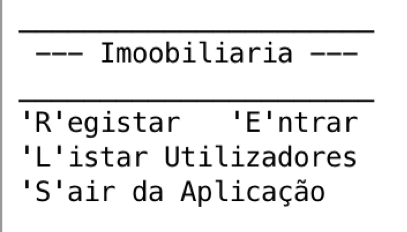
\includegraphics[scale=1] {imagens/Abertura.jpg}
\caption
\label
\end{figure}

\paragraph{Esta aplicação começa por apresentar ao utilizador um menu de abertura que lhe permite registar um vendedor ou um comprador ('R'egistar), iniciar sessão ('E'ntrar) e verificar a lista de utilizadores ('L'istar Utilizadores). Contém ainda a opção de sair do programa ('S'air).}

\newpage

\subsection{\textbf {Menu Registo}}

\begin{figure}[!htb]
\centering
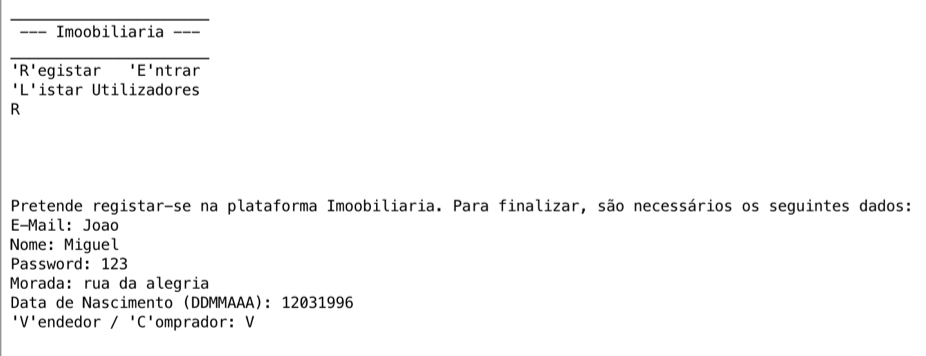
\includegraphics[scale=1] {imagens/MenuRegisto.jpg}
\caption
\label{}
\end{figure}

\paragraph{Na secção de registo do utilizador é necessário escrever o e-mail, nome, palavra-passe, morada, data de nascimento e indicar se é vendedor ('V') ou comprador ('C').}

\newpage

\subsection{\textbf {Menu Ínicio Sessão}}

\begin{figure}[!htb]
\centering
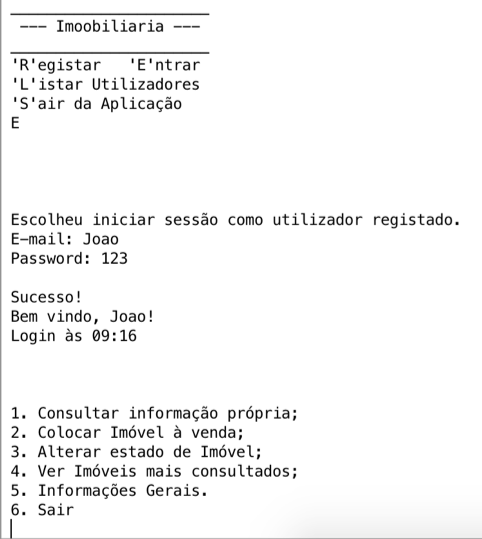
\includegraphics[scale=1] {imagens/123.jpg}
\caption
\label
\end{figure}

\paragraph{No menu de iniciar sessão é necessário ao utilizador indicar o e-mail e a correspondente palavra-passe e deste modo entrar na sua conta. Após o início de sessão aparece uma mensagem de boas vindas com o nome do utilizador, com a hora do login e ainda as opções que o usuário tem disponível.} 

\newpage

\subsection{\textbf {Erro Iniciar Sessão}}

\begin{figure}[!htb]
\centering
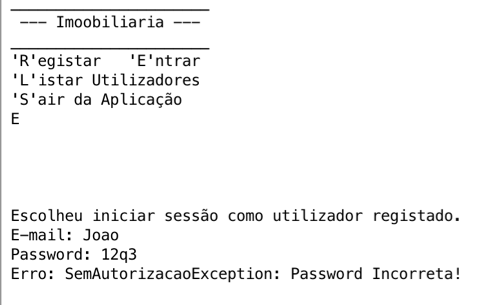
\includegraphics[scale=1] {imagens/ErroIniSessao.jpg}
\caption
\label
\end{figure}

\paragraph{Caso a palavra-passe esteja incorreta o utilizador não consegue iniciar sessão e é apresentada uma mensagem de erro.}

\newpage

\subsection{\textbf {Lista Utilizadores Registados}}

\begin{figure}[!htb]
\centering
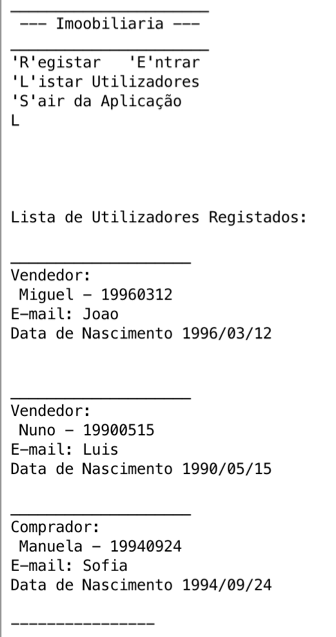
\includegraphics[scale=1] {imagens/ListaUsers.jpg}
\caption
\label
\end{figure}

\paragraph{No menu de abertura é possivel ainda selecionar a opção de visualização da lista de todos os usuários registados no sistema.}

\newpage

\subsection{\textbf {Após Iniciar Sessão}}

\paragraph{Após iniciar sessão encontramos um menu com diversas funções tais como a de consultar a própria informação, colocar um imóvel a venda, alterar o estado de um imóvel, verificar os imóveis mais consultados, ter acesso às informações gerais ou sair da aplicação.}

\begin{figure}[!htb]
\centering
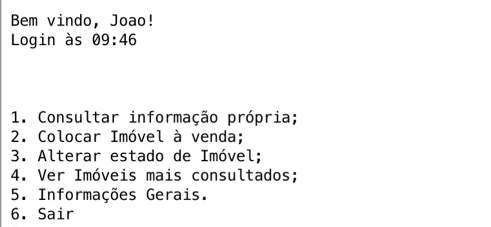
\includegraphics[scale=1] {imagens/123456.jpg}
\caption
\label
\end{figure}

\newpage

\subsection{\textbf{Menu Registo Imóvel}}

\begin{figure}[!htb]
\centering
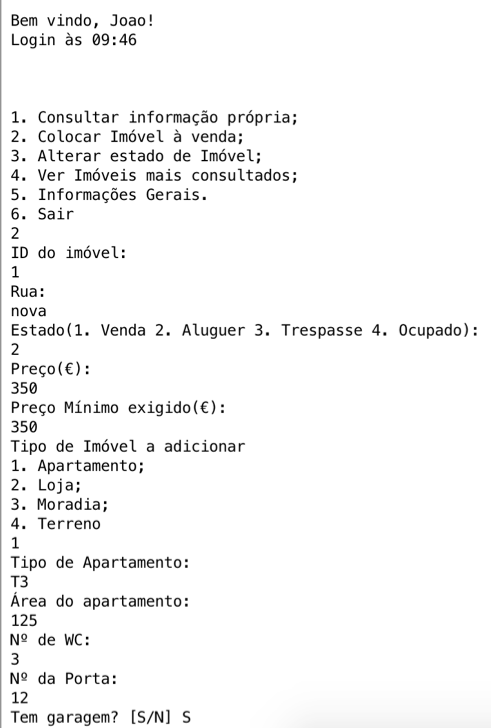
\includegraphics[scale=1] {imagens/12345.jpg}
\caption
\label
\end{figure}

\paragraph{Caso queiramos colocar um imóvel a venda aparecerá este menu que pede todo o tipo de informações refentes ao imóvel e o regista na base de dados.}

\newpage

\subsection{\textbf{Lista Geral Imoveis}}


\begin{figure}[!htb]
\centering
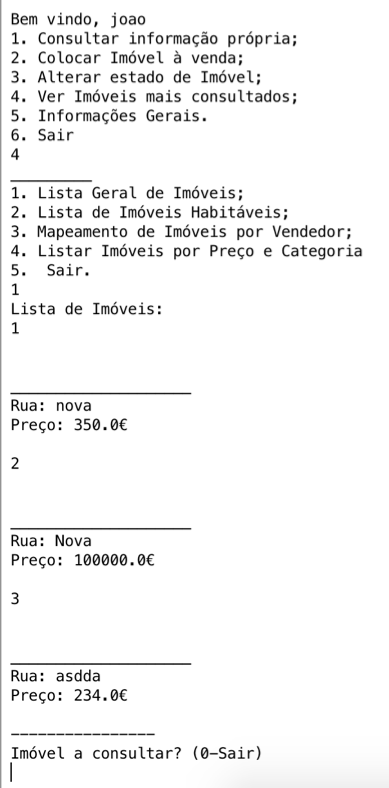
\includegraphics[scale=1] {imagens/MenuListaGeralImoveis1.jpg}
\caption
\label
\end{figure}

\paragraph{É possível ainda consultar a lista de imóveis registados na base de dados bem como as suas principais características e podendo selecionar o imóvel que pretende consultar mais detalhadamente.}

\newpage


\subsection{\textbf{Erro Preço Imóvel}}
\begin{figure}[!htb]
\centering
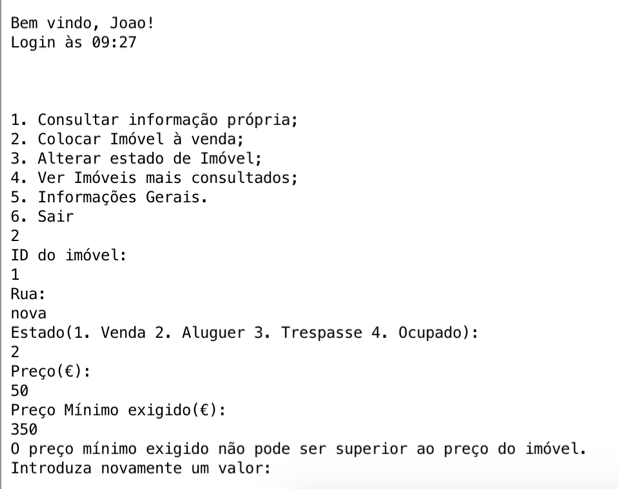
\includegraphics[scale=1] {imagens/1234.jpg}
\caption
\label
\end{figure}

\paragraph{Ainda no registo do imóvel quando o preço pedido é inferior ao preço mínimo pedido, a interface apresenta uma mensagem de erro e pede para introduzir novamente o valor.}

\newpage

\section{Conclusão}
\paragraph{Em suma, a realização do projeto correu dentro do esperado, tendo o nosso grupo atingido a maior parte dos objectivos definidos, elaborando as funções propostas para as principais funcionalidades do programa.}
\paragraph{Seria ainda possível incluir novos tipos de imóveis (caso fosse pedido) inserindo-os do mesmo modo como foram inseridos os outros, por exemplo, a moradia. Teríamos simplesmente de acrescentar mais uma classe com um construtor para o tipo de imóvel bem como os métodos de instância correspondentes as variáveis da classe e realizar o resto das alterações necessárias no código.}
\paragraph{Contudo, encontramos diversas adversidades embora tenhamos conseguido ultrapassar grande parte delas com a exceção da classe Leilão que não conseguimos elaborar. De resto, achamos que os nossos objectivos foram alcançados e da melhor maneira possível.}


\end{document}